\section{Hardware}

\begin{definition}[\textit{Sensor node}]
    A sensor node (or mote) is a device with several core capabilities:
    \begin{itemize}
        \item Sensing external phenomena, such as temperature, humidity, or pressure.
        \item Processing information collected by the sensors.
        \item Storing the gathered data.
        \item Communicating with other sensor nodes or external devices.
    \end{itemize}
\end{definition}
\noindent An actuator performs the following tasks: receiving input signals from control devices, processing and storing information, and acting on the industrial process, executing commands to modify conditions based on the input data.
\begin{figure}[H]
    \centering
    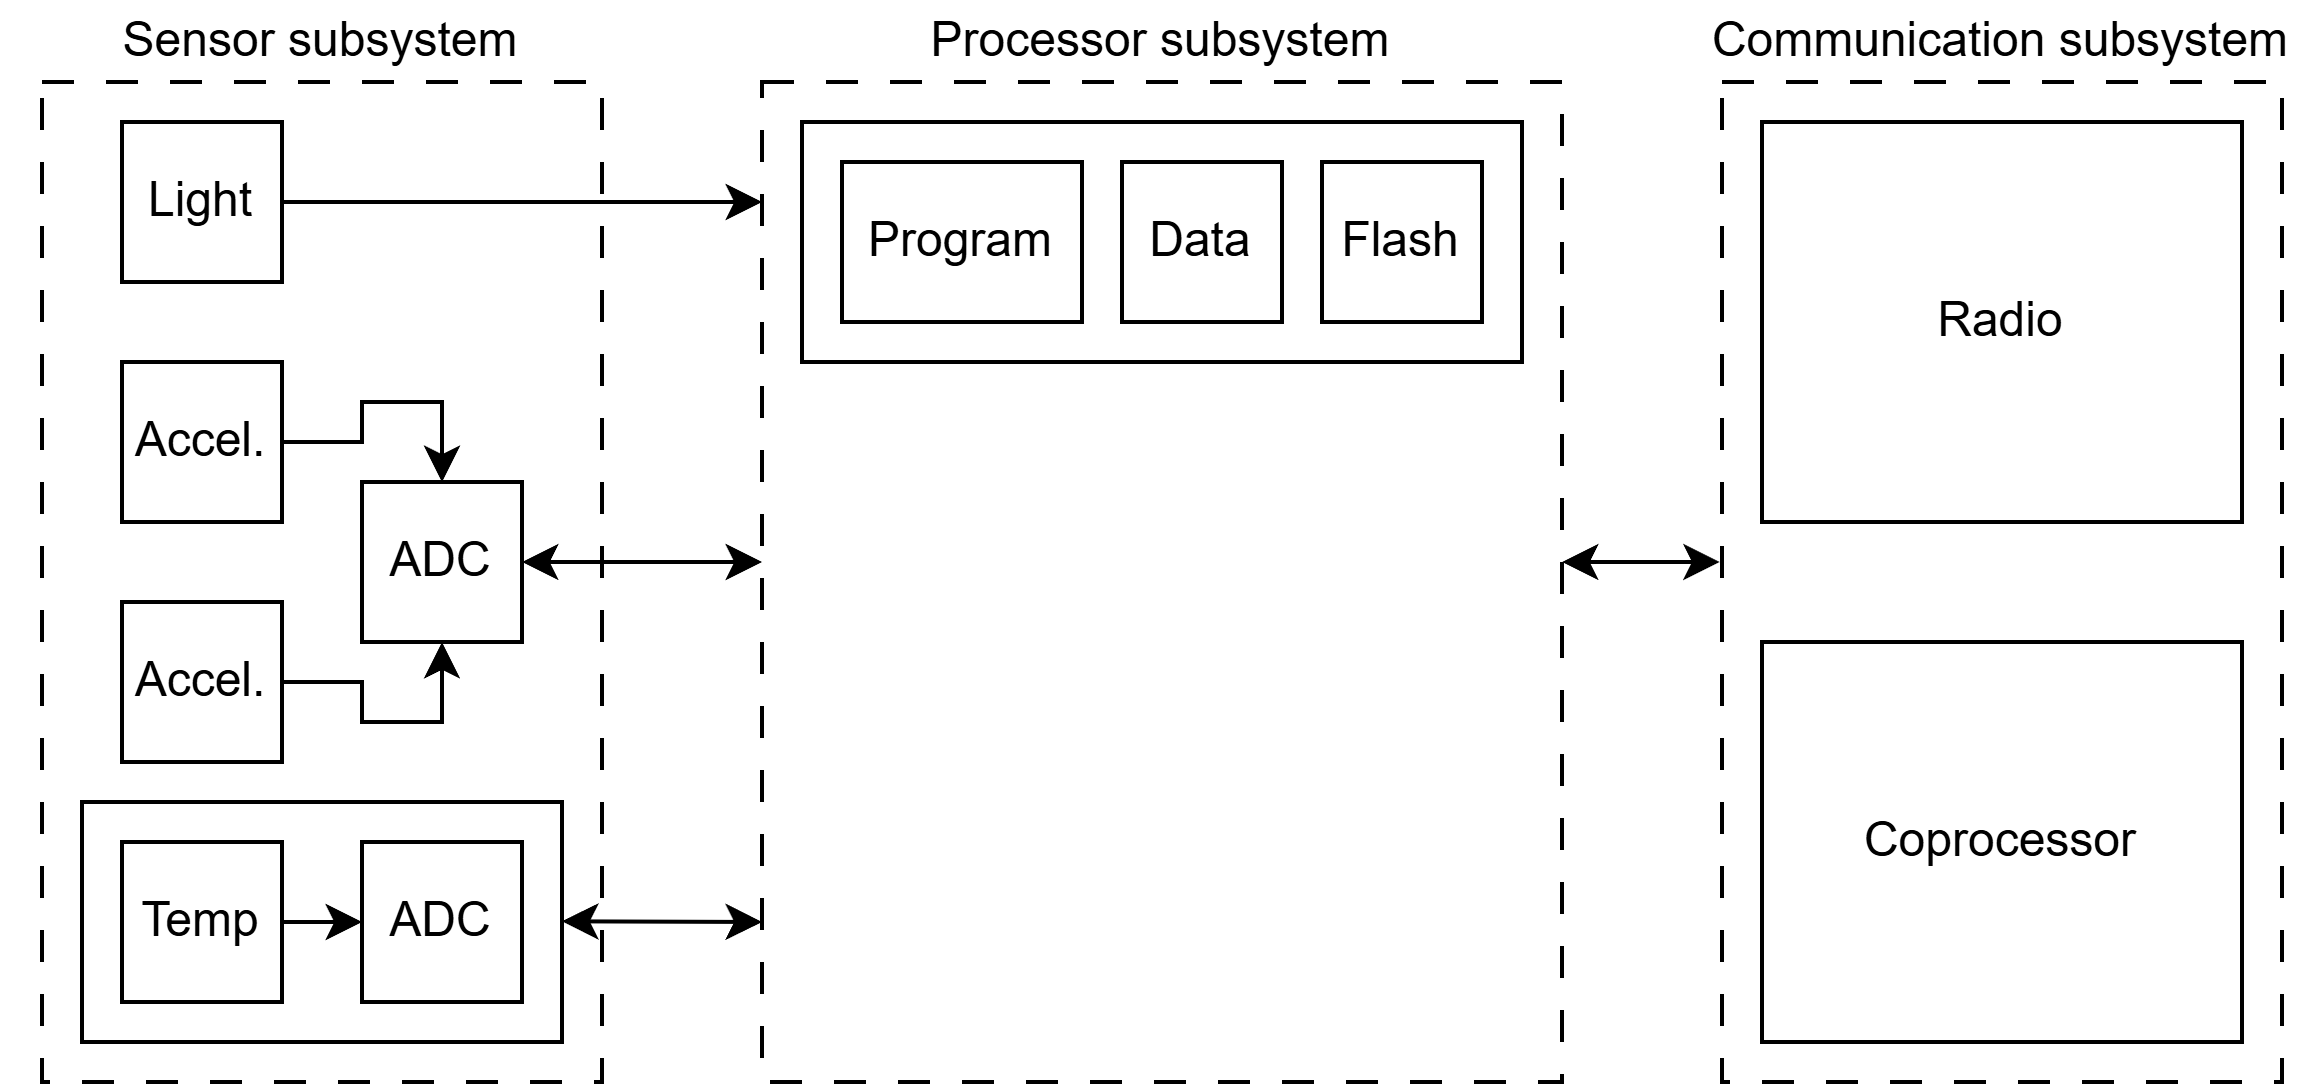
\includegraphics[width=0.75\linewidth]{images/sn.png}
    \caption{Sensor node architecture}
\end{figure}

\subsection{Processor}
The processor subsystem of a sensor node is often designed based on the SHARC architecture, though there are various alternatives for the individual components. 
These alternatives offer flexibility in terms of processing power, energy consumption, and other factors critical to specific use cases.
\begin{figure}[H]
    \centering
    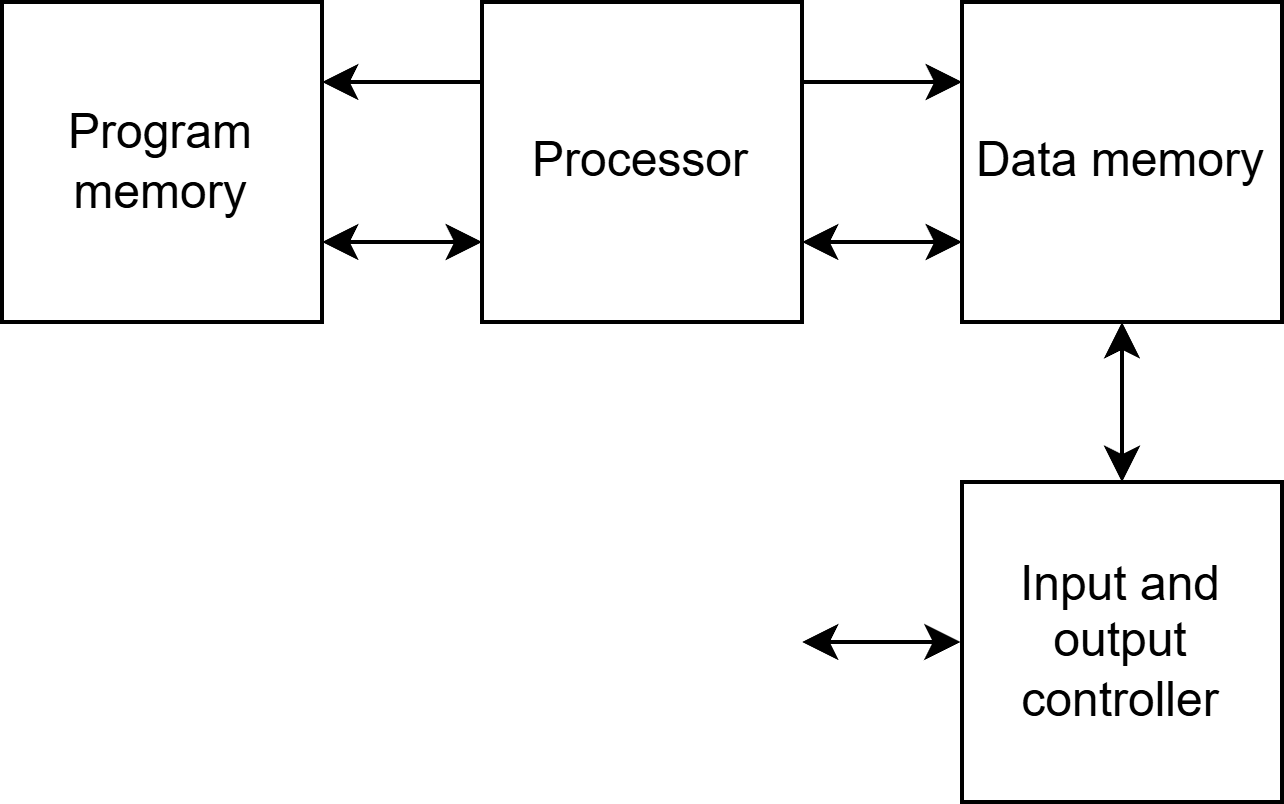
\includegraphics[width=0.5\linewidth]{images/pss.png}
    \caption{Processor architecture}
\end{figure}
A microcontroller is generally used as the processor in sensor nodes.
\begin{definition}[\textit{Microcontroller}]
    A microcontroller is a single integrated circuit designed for a specific application.
\end{definition}
A microcontroller is usually compose by a Central Processing Unit and a clock generator (oscillator with quartz timing crystals). 
It is usually equipped with RAM, flash memory and an EEPROM. 
It is connected with a serial BUS, I/O interfaces and analogic and digital converters. 
While microcontrollers are flexible and low-cost, they can compromise speed in certain use cases.

\begin{definition}[\textit{Digital Signal Processor}]
    A Digital Signal Processor is a specialized microprocessor optimized for processing discrete signals using digital filters.
\end{definition}
Digital Signal Processors excel at performing complex mathematical operations with extremely high efficiency. 
They can process hundreds of millions of samples per second, providing real-time performance. 
While they are well-suited for data-intensive operations, they are less flexible than microcontrollers.

\begin{definition}[\textit{Application Specific Integrated Circuit}]
    An Application Specific Integrated Circuit is a custom-designed integrated circuit tailored for a specific application.
\end{definition}
ASICS offer high speed and can be tailored for specific tasks, but they come with high development costs and limited flexibility once designed.

\begin{definition}[\textit{Field Programmable Gate Array}]
    A Field Programmable Gate Array has a high-level architecture similar to ASICs but allows for some degree of reconfigurability after manufacturing.
\end{definition}
Field Programmable Gate Arrays offer high-speed performance, supporting parallel programming, and moderate reconfigurability. 
However, they are more complex and costly than microcontrollers or Digital Signal Processors.












\subsection{Sensor}
\begin{figure}[H]
    \centering
    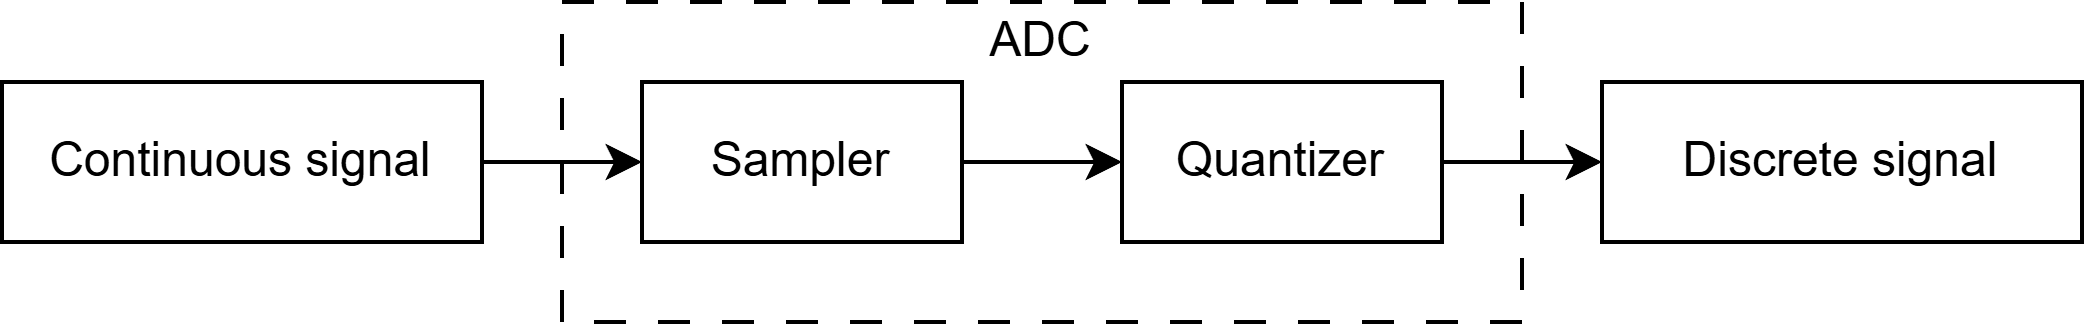
\includegraphics[width=0.75\linewidth]{images/adc.png}
    \caption{Analog to digital converter}
\end{figure}


\paragraph*{Sampling}
The Nyquist ADC technique involves reading a time-continuous signal at specific points in time. 
The sampling rate, or bandwidth, is the inverse of the sampling interval:
\[f_s=\dfrac{1}{T}\]
The key idea is that if the sampling frequency is properly set, the original signal can be losslessly reconstructed from its samples.
\begin{theorem}[Nyquist theorem]
    Given the signal bandwith $B$, we have that the sampling frequency must be chosen as:
    \[f_s=2B\]
\end{theorem}

\paragraph*{Quantization}
In quantization, the input voltage $V_{in}$ is approximated by a digital codeword. 
An ideal quantizer maps input to output with the smallest variation in the input causing a change in the codeword.
\begin{figure}[H]
    \centering
    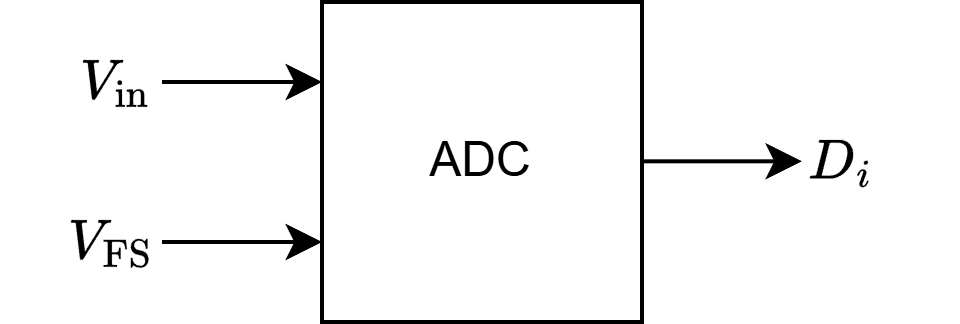
\includegraphics[width=0.5\linewidth]{images/quant.png}
    \caption{Quantization}
\end{figure}
The resolution refers to the smallest input variation that causes a change in the codeword:
\[\text{LBS}=\dfrac{V_{\text{FS}}}{2^n}\]
Here, $V_{\text{FS}}$ is the full-scale voltage and $n$ is the number of bits of resolution.

Quantization involves discretizing the continuous amplitude of the sampled signal. 
The quantization error occurs when the output voltage either overestimates or underestimates the input voltage. 
This error decreases as the resolution increases.

\paragraph*{Hardware possibilities}
The IoT hardware landscape is vast, fragmented, and heterogeneous, with a wide variety of options in terms of CPU types, connectivity, storage, and sensing peripherals. 
Many end-devices and sensors are now capable of running full operating systems, enabling more complex applications.

There is a clear distinction between the application layer and the hardware control layer, allowing for greater flexibility in how systems are designed and deployed.
However, there is also a battle between different types of operating systems in this space, including: commercial RTOS, open-source RTOS, and non-RTOS solutions.

\subsection{Processor power}
The power dissipation of the CPU is due to several factors, including:
\[P_{\text{p}}=P_{\text{dyn}}+P_{\text{sc}}+P_{\text{leak}}\]
Here, $P_{\text{dyn}}$ is the power consumed by the work done (dynamic power), $P_{\text{sc}}$ is the power lost due to short circuits, and $P_{\text{leak}}$ is the power lost due to leakage.
The dynamic power consumed during operation is given by:
\[P_{\text{dyn}}=CfV^2\]
Here, $C$ is the capacitance, $f$ is the frequency, and $V$ is the voltage. 

Local data processing is crucial in minimizing power consumption, especially in multi-hop networks, where power efficiency is key.

\subsection{Sensor and actuator power}
The absence of cables in wireless sensors and actuators means no wired power or connectivity. 
This presents unique challenges, especially in terms of energy efficiency, which becomes a must in these systems.

A sensor node typically operates with a limited power source, and its lifetime directly depends on the battery lifetime. 
The goal is to maximize the energy provided while minimizing the cost, volume, weight, and recharge requirements.
However, the problem arises when recharging or battery replacement becomes impractical or too expensive.

There are two main types of batteries used:
\begin{itemize}
    \item Primary batteries, which are not rechargeable.
    \item Secondary batteries, which are rechargeable, but only make sense when paired with some form of energy harvesting.
\end{itemize}

\paragraph*{Guidelines}
To extend battery life, one of the key strategies is to switch off the radio as soon as possible, since radios consume significant power. 
The power consumption of short-range wireless communication devices remains roughly the same whether the radio is transmitting, receiving, or just idle and listening for potential signals.

Circuit power is primarily dominated by the core components, rather than large amplifiers.
The radio must be listening to receive data, even if transmission is infrequent.
Listening is often continuous, meaning the total energy consumption is dominated by the power used during idle listening.

\paragraph*{Power cycle}
The power cycle of an IoT device consists of sleep and active states (wake-up/work). 
During the sleep state, power consumption is minimal, with only essential components running, resulting in some leakage.
The average power consumption is then defined as:
\[P_{\text{avg}}=f_{\text{sleep}}P_{\text{sleep}}+f_{\text{wakeup}}P_{\text{wakeup}}+f_{\text{work}}P_{\text{work}}\]
Here, $f_{\text{sleep}}$, $f_{\text{wakeup}}$, and $f_{\text{work}}$ are the fractions of time spent in sleep, wake-up, and work states, respectively.

The lifetime of the device is given by:
\[\text{lifetime}=\dfrac{\text{energy store}}{P_{\text{avg}}-P_{\text{gen}}}\]
Here, $P_{\text{gen}}$ is the power generated.

\paragraph*{Transmission consumption}
When data needs to be sent, the device first wakes up and then performs the actual transmission. 
The total energy consumption for this process is given by:
\[E_{tx}=P_{tx}(T_{wu}+T_{tx})+P_{0}T_{tx}\]
Here, $P_{tx}$ is the power consumed by the transmitter, $P_O$ is the output power of the transmitter,$T_{tx}$ is the time taken to transmit a packet, and $T_{wu}$ is the wake-up time.

\paragraph*{Reception consumption}
When the device needs to receive data, it first wakes up and then performs the reception. 
The total energy consumption in this case is:
\[E_{tx}=P_{rx}(T_{uw}+T_{rx})\]
Here, $P_{rx}$ is the power consumed by the receiver, $T_{rx}$ is the time taken to receive a packet, and $T_{wu}$ is the wake-up time.

\paragraph*{Emitted power}
The emitted power is often a tunable parameter, and it is generally considered good practice to set it to the lowest value that still allows for reliable reception. 
The quality of the reception process is typically measured using metrics like:
\begin{itemize}
    \item \textit{Bit Error Rate}: the fraction of bits that are incorrectly received. 
    \item \textit{Packet Error Rate}: the fraction of packets that are not received correctly.
\end{itemize}
The relationship between BER and PER, for a packet of length $l$ with independent errors, is given by:
\[\text{PER}=1-(1-\text{BER})^l\]
Both BER and PER are influenced by the level of noise in the transmission and reception channels, which in turn is determined by the transmitted and received power. 
The Signal-to-Interference-plus-Noise Ratio is a key factor in determining this quality, and is calculated as:
\[\text{SINR}=10\log_{10}\left(\dfrac{P_{\text{recv}}}{N_0+\sum_{i=1}^{k}I_i}\right)\]
Here, $N_0$ is the thermal noise (KTB), $P_{\text{recv}}$ is the received power, and $I_i$ are the interference contributions from other signals.
Given the SINR and the specific modulation of the channel, BER can be computed.

\paragraph*{Receiver sensitivity}
Each receiver is characterized by a sensitivity parameter, which is the minimum input signal power required for the receiver to demodulate the data correctly. 
Knowing this sensitivity, the required emitted power at the transmitter can be determined by inverting the propagation law of the communication channel.

\paragraph*{Sensor power}
The power consumption due to sensing is highly dependent on the type of sensor used. 
A rough model for the power consumption of an Analog-to-Digital Converter can be expressed as:
\[P_s\sim f_s2^n\]
Here, $f_s$ is the sampling frequency, and $n$ is the resolution of the ADC (in bits).

\subsection{Design guidelines}
Avoid full operation all the time. 
If there's no active task, switch to power-safe modes to preserve battery life.

Use power-aware operating systems that dim displays, enter sleep mode during idle times, and implement power-aware scheduling. 
Enable radios to forward packets at a lower power level while keeping the rest of the node in a sleep mode.
Take advantage of performance-energy trade-offs within the communication subsystem by optimizing neighbor coordination and selecting appropriate modulation schemes.